\chapter{Mixed-Bag Solver Overview}

This thesis' Mixed-Bag Solver supports Type~1, Type~2, and Mixed-Bag Puzzles.  It consists of five distinct stages namely: segmentation, stitching piece solving, hierarchical clustering of segments, seed piece selection, and final assembly.  The flow of the algorithm is shown in Figure~\ref{fig:multipuzzleSolverArchitecture}.

The following subsections describe each of the components solver architecture.  It also discusses the assembler which is an independent but associated component of the architecture.

\begin{figure}[ht!]
	\centering
		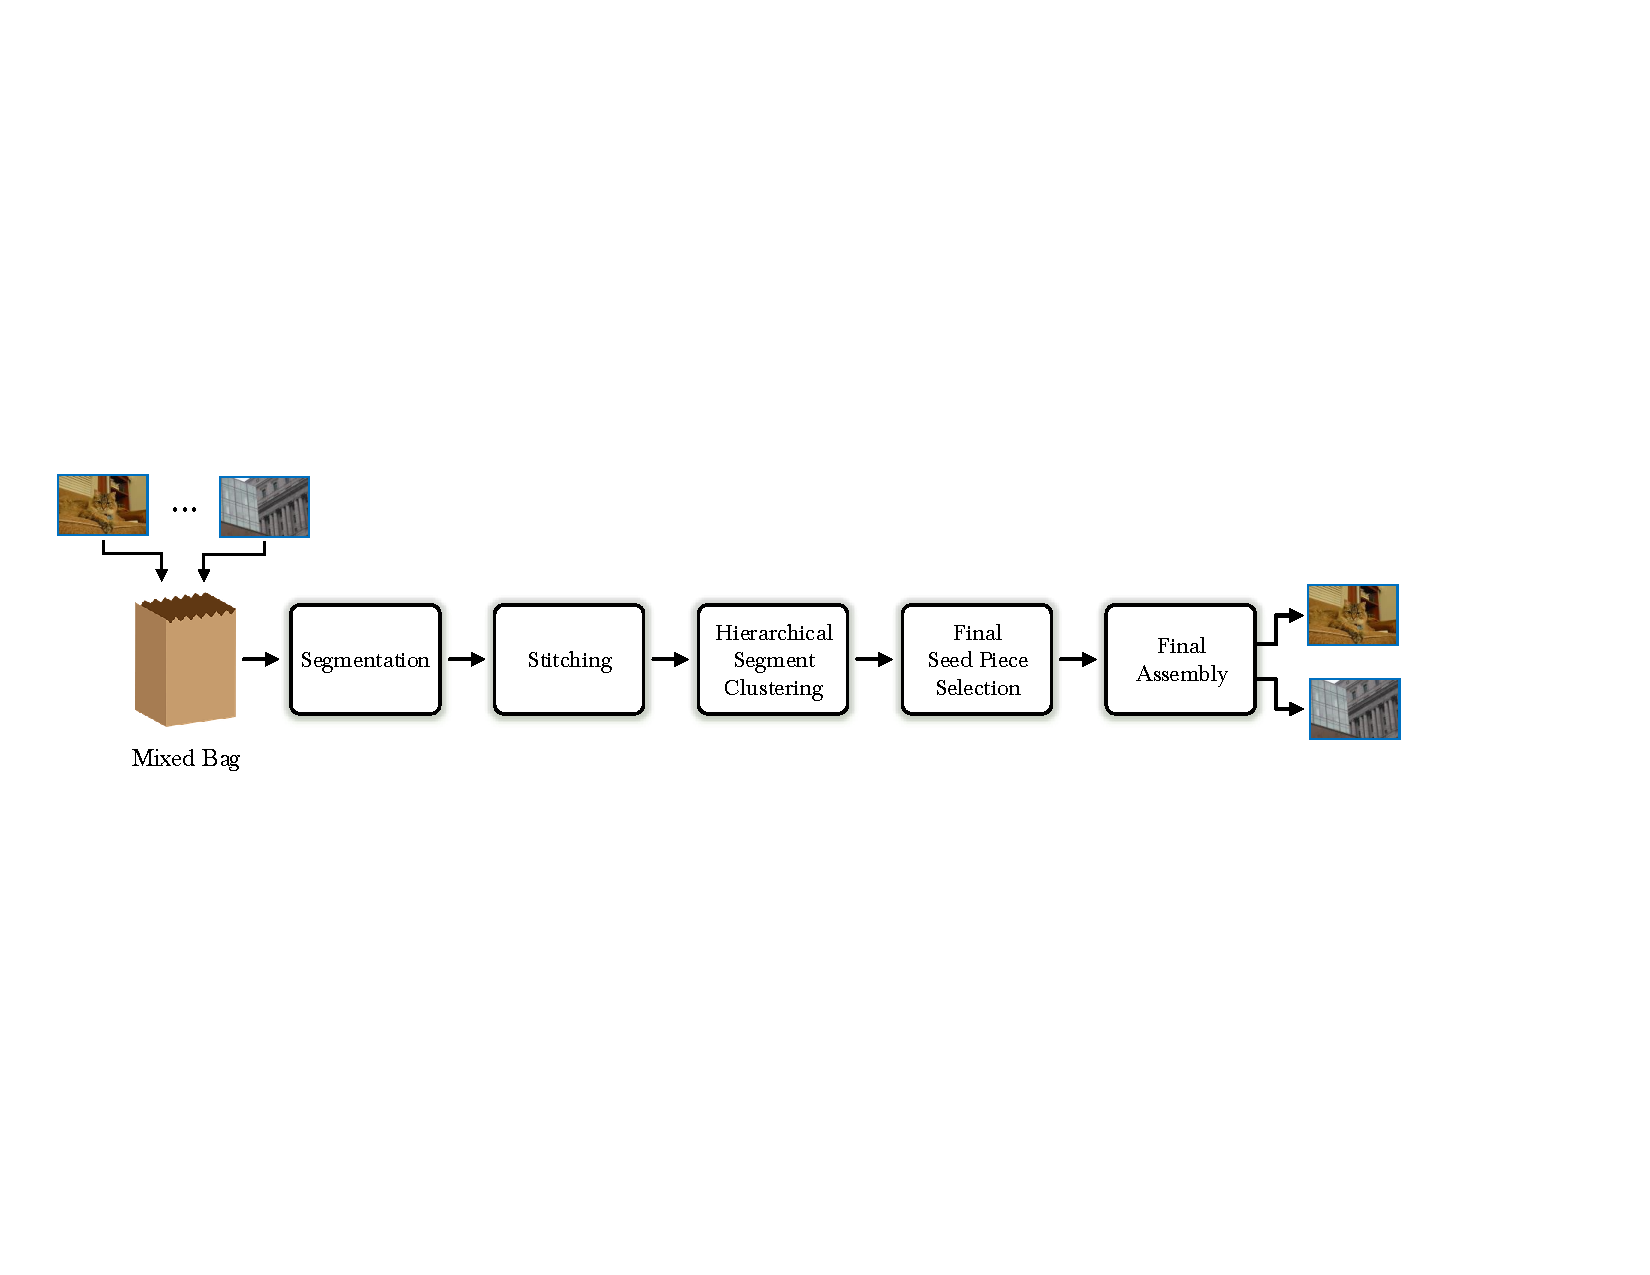
\includegraphics[width=1.0\textwidth]{images/cropped_algorithm_structure_overview.pdf}
	\caption{Components of the Mixed-Bag Puzzle Solver}\label{fig:multipuzzleSolverArchitecture}
\end{figure}

\section{Assembler}\label{sec:SolverAssembler}

The role of the assembler assigns the placement (and optionally rotation) of the puzzle pieces in the solved puzzle.  This solver architecture is largely independent of the assembler used.  Hence, as assemblers improve, they can be incorporated into this solver to improve the overall performance.  The same also applies if particular assembler(s) perform better for particular types of puzzles.  This enables significant flexibility to balance competing concerns, while maintaining upgradability.

For all experiments in this thesis, we used the solver proposed by Paikin \& Tal \cite{paikin2015}.  It was selected because it the current state-of-the-art.  What is more, since it supports mixed bag puzzles, it can be used for direct comparison of performance.

\section{Segmentation}\label{sec:Segmentation}

As the first stage in the Mixed-Bag Solver, segmentation takes as input only the bag of puzzle pieces created from the original images; unlike all other solvers to date, this algorithm takes no other inputs.  The role of stage is to provide structure to the unordered input.  This is done by partitioning the pieces into disjoint sets, referred to here as segments.  These segments are groups of puzzle pieces where there is a high degree of confidence that the pieces are assembled correctly.

Algorithm~\ref{alg:segmentation} outlines the basic segmentation framework.  The algorithm is iterative and will have one or more rounds.  In each round, all pieces that have not yet been assigned to a segment are assembled as if they all belong to a single ground truth image.  This is done as it eliminates the need to make any assumptions regarding the input at this early stage of the solver.  While it may lead to a single puzzle being divided into multiple segments, these segments can be merged together later in a later stage of the solver.

After the single puzzle is assembled in each round, the solved puzzle is then divided into segments; the procedure for this is described in Section~ \label{sec:segmentPuzzle}.  Assuming the largest segment exceeds the minimum allowed size\footnote{This thesis found that a minimum segment size of 7 provided the best balance between solution quality and algorithm execution time.}, it is passed to the next stage of the Mixed-Bag Solver.  

The term ``\textit{$\alpha$}'' in Algorithm~\ref{alg:segmentation} defines which segments other than the largest one constructed puzzle are immediately passed to the next solver stage.  In this thesis, \textit{$\alpha$} was set to 0.5, meaning any segment that was at least half the size of the largest segment in that round (and larger than the minimum segment size) is saved.  This scalar value provides sufficient balance between ensuring the largest segments for analysis with limiting the execution time of this stage.

Once a piece is assigned to a saved segment, it is removed from the set of unassigned pieces.  Hence, those pieces will not be placed in the next segmentation round.  Segmentation continues until all pieces have been assigned to sufficiently large segments, or no segment exceeds the minimum allowed segment size.

\begin{algorithm}
\caption{Pseudocode for the Segmentation Algorithm}\label{alg:segmentation}
\begin{algorithmic}[1]
\Procedure{Segmentation}{$all\_pieces$}
    \State $\textit{saved\_segments} \gets \{ \}$
    \State $\textit{unassigned\_pieces} \gets \{ \textit{all\_pieces} \}$
    \Do
        \State $\textit{solved\_puzzle} \gets \textbf{run\_single\_assembly}(\textit{unassigned\_pieces})$
        \State $\textit{solved\_segments} \gets \textbf{segment\_puzzle}(\textit{solved\_puzzle})$
        \State $\textit{max\_segment\_size} \gets \text{maximum size of segment in } \textit{solved\_segments}$
        \ForEach{$\textit{segment} \in \textit{solved\_segments}$}
            \If{$|\textit{segment}| \text{>} \alpha \times \textit{max\_segment\_size}$}
                \State $\text{add } \textit{segment} \text{ to } \textit{saved\_segments}$
                \State $\text{remove pieces in } \textit{segment} \text{ from } \textit{unplaced\_pieces}$
            \EndIf
        \EndFor
    \doWhile{$\textit{max\_segment\_size} \text{>} \textit{smallest\_allowed} \textbf{ and } |\textit{unplaced\_pieces}| \text{>} 0$}
\EndProcedure
\end{algorithmic}
\end{algorithm}

\subsection{{segment\_puzzle} Procedure}\label{sec:segmentPuzzle}

The \texttt{segment\_puzzle} procedure shown in Algorithm~\ref{alg:segmentPuzzle} is adapted from the kernel growing segmentation procedure modified by Pomeranz \textit{et al.}, where it was shown to have greater than 99.7\% accuracy identifying genuine neighbors \cite{pomeranz2011}. The kernel of each segment is a single seed piece.

\begin{algorithm}
\caption{Pseudocode for the segment\_puzzle Function}\label{alg:segmentPuzzle}
\begin{algorithmic}[1]
\Procedure{segment\_puzzle}{$solved\_puzzle$}
    \State $\textit{solved\_segments} \gets \{ \}$
    \State $\textit{unassigned\_pieces} \gets \{ \text{all pieces in } \textit{solved\_puzzle} \}$
\item[]
    \While{$|\textit{unassigned\_pieces}| \text{>} 0$}
        \State $\textit{segment} \gets \text{ new empty segment}$
        \State $\textit{seed\_piece} \gets \text{next piece in } \textit{unassigned\_pieces}$
        \State $\textit{queue} \gets [\textit{seed\_piece}]$
\item[]
        \While{$|\textit{queue}| \text{>} 0$}
            \State $\textit{piece} \gets \text{next piece in }\textit{queue}$
            \State $\text{add } \textit{piece} \text{ to } \textit{segment}$
\item[]
            \ForEach{$\textit{neighbor\_piece} \text{ of } \textit{piece}$}
            	\If{$\textbf{is\_best\_buddies}(\textit{neighbor\_piece}, \textit{piece})$}
            		\State $\text{add } \textit{neighbor\_piece} \text{ to } \textit{queue}$
            		\State $\text{remove } \textit{neighbor\_piece} \text{ from } \textit{unassigned\_pieces}$
            	\EndIf
            \EndFor
        \EndWhile
\item[]
        \State $\textit{articulation\_points} \gets \textbf{find\_articulation\_points}(\textit{segment})$
        \State $\text{remove } \textit{articulation\_points} \text{ from } \textit{segment}$
\item[]
		\State $\textit{disconnected\_pieces} \gets \textbf{find\_disconnected\_pieces}(\textit{segment},\textit{seed\_piece})$        
        \State $\text{remove } \textit{disconnected\_points} \text{ from } \textit{segment}$
\item[]
        \State $\text{add } \textit{articulation\_points} \text{ and } \textit{disconnected\_pieces} \text{ to } \textit{unassigned\_pieces}$
    \EndWhile
\EndProcedure
\end{algorithmic}
\end{algorithm}

Whenever a piece is added to a segment, it is removed from the set of unassigned pieces. What is more, the algorithm check's all pieces directly adjacent to the added piece.  If the adjacent piece and the added piece are ``best buddies'' (i.e., each is more similar to the other on their respective sides than they are to any other piece as defined by \cite{pomeranz2011} and \cite{paikin2015}), then the adjacent piece is also added to the segment.  This process continues until no there are no pieces adjacent to a segment member that fulfill the best buddy criteria.

If Pomeranz \textit{et al.}'s original segmentation algorithm is used for Mixed-Bag puzzles, two correctly assembled segments from different input puzzles can be merged into a single segment.  This is usually in the form of narrow bridges no wider than a single piece. This necessitates that each segment goes through post-processing to identify and remove these single point bridges; the procedure for doing this is described in Section~\ref{sec:ArticulationPoints}.  

Once these single piece bridges have been broken, one or more pieces become disconnected from the segment.  These pieces are then returned to the set of unassigned pieces to be assigned to a different segment.  At the end of segment, each piece in the puzzle will be assigned to exactly one segment.

\subsection{Articulation Points}\label{sec:ArticulationPoints}

A segment can be model as a single connected graph, with the vertices being the puzzle pieces and the edges being the best buddy relationships.  An articulation point is any vertex (\textit{i.e.}, puzzle piece) whose removal increases the number of connected components.  The Mixed-Bag Solver uses the algorithm proposed by \ref{cormen} for identifying articulation points.  While most implementations of this algorithm are recursive, this thesis instead uses an iterative approach as segment can be several thousand pieces in sizes.  As such, a recursive implementation is prone to stack overflows.

\section{Stiching Piece Solving}\label{sec:stitchingPieceSolving}

As defined previously, a segment represents a partial assembly where there is a particularly high degree of confidence that the placement is correct. During the segmentation stage, puzzle pieces from a single ground truth image segment may be partitioned into multiple segments. If two segments are similar, it is likely that if one segment is allowed to grow that it would eventually merge with its adjacent segment.  However, uncontrolled segment expansion can cause a segment to grow beyond the boundaries of its ground truth image and merge with a segment from a different input image.  This thesis controls segmentation growth through the use of multiple ``mini solvers,'' which each have a ``stitching piece'' as their seed.  The output from these mini solvers are used to determine inter-segment similarity as described in the following subsection.

\subsection{Stitching Pieces}

As the name indicates, stitching pieces are a set of pieces whose role is to assisting in the ``stitching'' together of associated segments.  Since segments are disjoint, a segment will need to grow in order to join with another segment.  

Stitching pieces should be near the edge of a segment to increase the likelihood of growth to a neighboring segment.  However,  if they are placed too close to the edge of the segment, the algorithm may find erroneous segment pairings that are not meaningful.  To determine the distance each piece is from the edge of the segment, this thesis uses an iterative boundary tracing technique shown in Algorithm~\ref{alg:stitchingPieceDistance}.

The algorithm begins by finding set of puzzle locations adjacent to pieces in the segment that are not filled by segment members.  These locations represent the .

\begin{algorithm}
\caption{Pseudocode for the segment\_puzzle Function}\label{alg:segmentPuzzle}
\begin{algorithmic}[1]
\Procedure{segment\_puzzle}{$solved\_puzzle$}
    \State $\textit{solved\_segments} \gets \{ \}$
    \State $\textit{unassigned\_pieces} \gets \{ \text{all pieces in } \textit{solved\_puzzle} \}$
\item[]
    \While{$|\textit{unassigned\_pieces}| \text{>} 0$}
        \State $\textit{segment} \gets \text{ new empty segment}$
        \State $\textit{seed\_piece} \gets \text{next piece in } \textit{unassigned\_pieces}$
        \State $\textit{queue} \gets [\textit{seed\_piece}]$
\item[]
        \While{$|\textit{queue}| \text{>} 0$}
            \State $\textit{piece} \gets \text{next piece in }\textit{queue}$
            \State $\text{add } \textit{piece} \text{ to } \textit{segment}$
\item[]
            \ForEach{$\textit{neighbor\_piece} \text{ of } \textit{piece}$}
            	\If{$\textbf{is\_best\_buddies}(\textit{neighbor\_piece}, \textit{piece})$}
            		\State $\text{add } \textit{neighbor\_piece} \text{ to } \textit{queue}$
            		\State $\text{remove } \textit{neighbor\_piece} \text{ from } \textit{unassigned\_pieces}$
            	\EndIf
            \EndFor
        \EndWhile
\item[]
        \State $\textit{articulation\_points} \gets \textbf{find\_articulation\_points}(\textit{segment})$
        \State $\text{remove } \textit{articulation\_points} \text{ from } \textit{segment}$
\item[]
		\State $\textit{disconnected\_pieces} \gets \textbf{find\_disconnected\_pieces}(\textit{segment},\textit{seed\_piece})$        
        \State $\text{remove } \textit{disconnected\_points} \text{ from } \textit{segment}$
\item[]
        \State $\text{add } \textit{articulation\_points} \text{ and } \textit{disconnected\_pieces} \text{ to } \textit{unassigned\_pieces}$
    \EndWhile
\EndProcedure
\end{algorithmic}
\end{algorithm}

Algorithm~\ref{} has $O(n)$ time complexity where $n$ is the number of pieces in the segment.  What is more, the algorithm is robust enough to handle voids within a segment as well as potential necking within the segment where two large segment components are joined by a narrower bridge.

\subsection{Stitching Pieces}

If stitching pieces are placed to close together, the solver will perform many redundant solvings.  While this may not have a deleterious effect on the solver output, it can significantly increase the execution time of this stage.  In contrast, if stitching pieces are placed too far apart, subtle segment pairings may be missed.  To achieve 

Figure~\ref{} shows an original image along with an segment found during the segmentation.  This figure also shows the location of the stitching pieces (denoted with a white cross).  

\subsection{Quantifying Inter-Segment Similarity}



\section{Hierarchical Clustering of Segments}

\subsection{The Similarity Matrix}

\section{Selection of Starting Pieces}

\section{Final Assembly}